\cleardoublepage
\section{Grundlagen}
\subsection{Simulationsumgebung}
Die Simulationsumgebung wurde von der \atlas entwickelt und wird für diese Arbeit zur Verfügung gestellt [Abb. \ref{screenSim}].
In der Simulation wird die Fahrzeugsensorik und Aktuatorik simuliert (siehe Kapitel \ref{sec_auvSimGrundlage}). Außerdem wird noch eine grundlegende Wasserbewegung erzeugt, die durch Parametrisierung verändert werden kann.\\

Die Umgebung an sich besteht aus \textit{wrl}-Dateien, in denen die Welt mit \textit{\gls{vrml}} beschrieben wird. Diese einzelnen Dateien werden in der \textit{main.wrl} zusammengefügt. Bereits vorhanden sind \textit{wrl}-Dateien für das \gls{auv}, in denen die Realvorlage maßstabsgetreu nachgebildet wird sowie ein Generator zum Erstellen zufallsgenerierter Meeresböden in \textit{wrl}. Die Objekte, die in der Arbeit verfolgt werden sollen, wurden in \textit{\gls{vrml}} modelliert und dann als Unterknoten in der \textit{main.wrl} hinzugefügt.\\
Die Simulation basiert auf der \matlab Simulink 3D Animation Toolbox, somit stehen auch weitere \matlab -Toolboxen zur Verfügung. 
\begin{figure}[H]
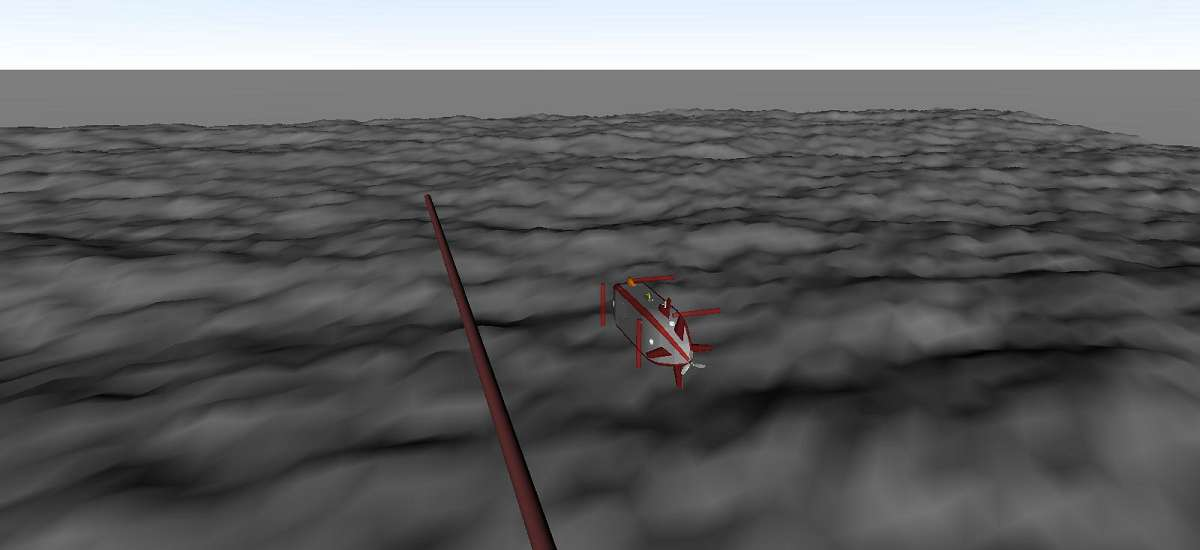
\includegraphics[width=\textwidth,scale=0.5]{Einleitung/ScreenshotSimulation.jpg}
\caption[Screenshot der Simulationsumgebung]{Screenshot der Simulationsumgebung mit dem \gls{auv}, einem Testobjekt und dem generierten Meeresboden}
\label{screenSim}
\end{figure}
\subsection{AUV-Simulation}
\label{sec_auvSimGrundlage}
Das simulierte \gls{auv} wurde von der \atlas auf Grundlage eines der eigenen \gls{auv}s entwickelt. Zu dieser Simulation gehören die bereits erwähnten \textit{wrl} Dateien sowie eine Simulation der Fahrzeugaktuatorik und -sensorik in \matlab Simulink. Es werden die für die Steuerung benötigte Schnittstelle in Form von Wegpunkten ($x$ und $y$ Koordinaten) und eine Schnittstelle für die innere Sensorik des \gls{auv}s bereitgestellt. Die für diese Arbeit wichtigen Informationen aus der inneren Sensorik bestehen aus der \gls{pose} des \gls{auv}s in der Welt in Form von geografischen Koordinaten, der Höhe über dem Meeresboden und den \gls{roll}-, \gls{pitch}- und \gls{yaw}-Werten.\\
Für die Steuerung wird ein \texttt{\gls{lanefollow}} verwendet, der das Fahrzeug auf einer Linie zwischen einem neuen und einem alten Wegpunkten führt. Für die Höhenkontrolle werden zwei Steuerungsmodi zur Verfügung gestellt. Zum einen die Fahrt auf Tiefe unter der Wasserobefläche oder Höhe über Meeresboden. Für diese Arbeit wird die Fahrt auf Höhe über dem Meeresboden gewählt, da die \gls{transform} von Pixelkoordinaten in Kamerakoordinaten am zuverlässigsten in dem Abstand zum Objekt funktioniert, in dem auch die Kamerakalibrierung durchgeführt wurde. Änderungen der Höhe können zu leichten Fehlern in der Positionsbestimmung führen. Jedoch sind diese Fehler bei realistischen Höhenunterschieden von einigen Metern nicht ausschlaggebend für die Ergebnisse der Arbeit.

Am Bug des \gls{auv}s befindet sich eine Kamera, die zentral nach unten ausgerichtet ist. Das Sichtfeld beträgt dabei 45$^\circ$ bei einer Auflösung von 640x480 Pixeln.
\subsection{Koordinatensysteme}
\label{sec_coordsystems}
Im Folgenden werde ich die Koordinatensysteme beschreiben, in denen Koordinaten angegeben werden. Hierbei wird von einer Tangentialebene an der WGS84-Kugel\footnote{https://confluence.qps.nl/pages/viewpage.action?pageId=29855173} verschoben auf den Meeresboden ausgegangen, da nur hinreichend kleine Operationsgebiete des \gls{auv}s betrachtet werden, sodass die Erdkrümmung keine Auswirkung hat.
\subsubsection{Bild und Kamera}
\label{sec_img_cam_coords}
Das Bildkoordinatensystem [Abb. \ref{imageKoords}] beschreibt die Anordnung der Pixel im Bild als 2D-Koordinaten. Der Ursprung ist immer die linke obere Bildecke. Ich gehe davon aus, dass das Bildkoordinatensystem immer auf der Meeresbodenebene liegt. Diese Annahme ist wichtig für die \glspl{transform} [Kapitel \ref{sec_transformations}].
\todo{schönere grafik evtl selber machen}

\begin{figure}[H]
	\centering
	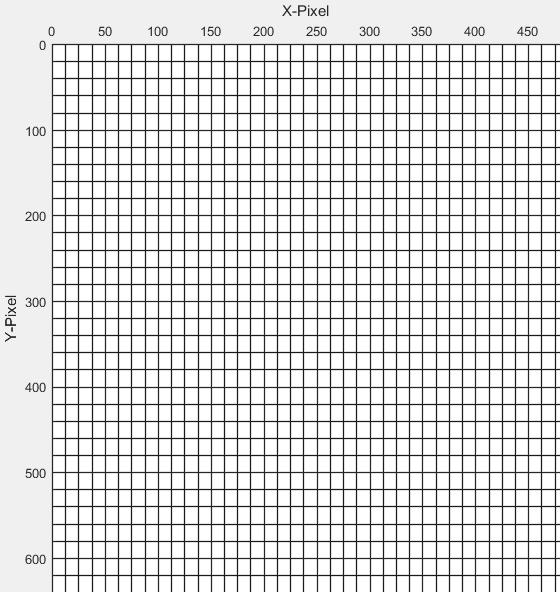
\includegraphics[scale=1]{Einleitung/imageCoords2.jpg}
	\caption[Das Bildkoordinatensystem]{Anordnung der 2D-Pixelkoordinaten. Ursprung liegt in der linken oberen Bildecke. Die X-Achse bildet die Bildspalten und die Y-Achse die Bildzeilen ab.}
	\label{imageKoords}
\end{figure}
Das Kamerakoordinatensystem [Abb. \ref{CamKoords}] beschreibt das dreidimensionale Koordinatensystem mit Ursprung im Mittelpunkt der Kameralinse. Die Kamera befindet sich 25 cm unter und 1,3 m vor dem Fahrzeugmittelpunkt.
\todo{bessere qualität}
\begin{figure}[H]
	\centering
	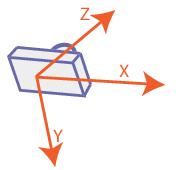
\includegraphics[scale=1]{Einleitung/camCoords.jpg}
	\caption[Das Kamerakoordinatensystem]{Das Kamerakoordinatensystem. Ursprung des Systems liegt im Mittelpunkt der Kameralinse. Die X-Achse bildet die Bildspalten und die Y-Achse die Bildzeilen im Raum ab. Die Z-Achse zeigt in Blickrichtung der Kamera.}
	\label{CamKoords}
\end{figure}

\subsubsection{Body}
Das Body-Koordinatensystem beschreibt das Koordinatensystem relativ zum \gls{auv}-Mittelpunkt [Abb. \ref{Abb. 1}].
Der Ursprung wird hierbei durch den Massenschwerpunkt des \gls{auv}s bestimmt.
Das Koordinatensystem entspricht dem klassischen nautischen Koordinatensystem, dem North-East-Down Koordinatensystem (vgl. Kapitel 2 in \texttt{Unmanned rotorcraft systems} \cite{cai2011unmanned})
\begin{figure}[H]
	\centering
	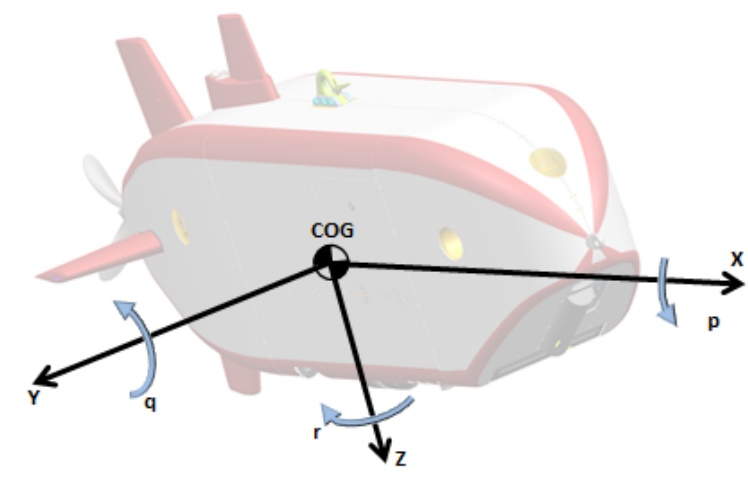
\includegraphics[scale=0.7]{Einleitung/bodyKoords.jpg}
	\caption[Das Body-Koordinatensystem]{Das Body-Koordinatensystem mit Massenschwerpunkt (\textit{cog}) des \gls{auv}s. Die X-Achse zeigt frontal voraus, die Y-Achse Richtung Steuerbord und die Z-Achse zeigt nach unten. \textit{p} \textit{r} und \textit{q} beschreiben die Neigungswinkel und Rotationsrichtung an den jeweiligen Achsen (vgl. Abb. \ref{Abb. 2})}
	\label{Abb. 1}
\end{figure}

Die Neigungswinkel (\gls{roll}-\gls{pitch}-\gls{yaw}) werden wie in [Abb. \ref{Abb. 2}] im Body Koordinatensystem angegeben.
%\begin{figure}[H]
%	\centering
%	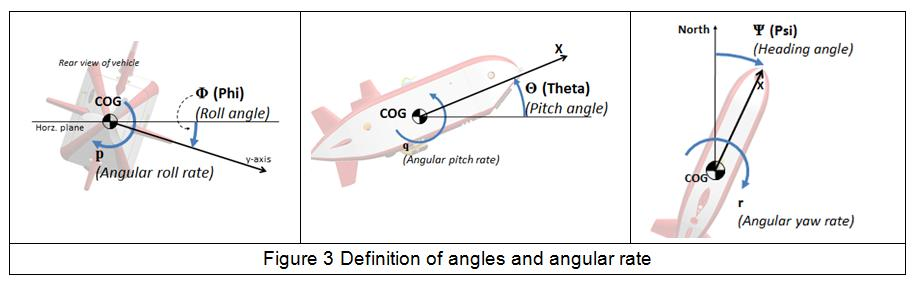
\includegraphics[scale=0.7]{Einleitung/rollPitchYaw.jpg}
%	\caption[Die Neigungswinkel im Body-Koordinatensystem]{Die Neigungswinkel am \gls{auv}. Phi beschreibt den \gls{roll} Winkel um den Massenschwerpunkt (\textit{cog}) und p die dazugehörige \textit{roll rate},  Theta beschreibt den \gls{pitch} Winkel um den Massenschwerpunkt (\textit{cog}) und q die dazugehörige \textit{roll rate} und  Psi beschreibt die Ausrichtung des \gls{auv}s im Bezug zur Nordrichtung.}
%	\label{Abb. 2}
%\end{figure}

\begin{figure}[H]
\begin{tabular}{ccc}
\subfloat[]{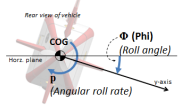
\includegraphics[width=0.33\textwidth]{/Einleitung/roll.png}}&
\subfloat[]{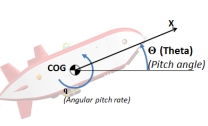
\includegraphics[width=0.33\textwidth,height=0.2\textheight]{/Einleitung/pitch.png}}&
\subfloat[]{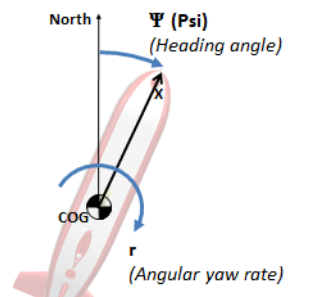
\includegraphics[width=0.33\textwidth,height=0.2\textheight]{/Einleitung/yaw.png}}
\end{tabular}
\caption[Die Neigungswinkel im Body-Koordinatensystem]{Die Neigungswinkel am \gls{auv}. Phi beschreibt den \gls{roll} Winkel um den Massenschwerpunkt (\textit{cog}) und p die dazugehörige \textit{roll rate},  Theta beschreibt den \gls{pitch} Winkel um den Massenschwerpunkt (\textit{cog}) und q die dazugehörige \textit{roll rate} und  Psi beschreibt die Ausrichtung des \gls{auv}s im Bezug zur Nordrichtung.}
\label{Abb. 2}
\end{figure}
\subsubsection{\matlab und \gls{vrml} (World)}
Abbildung \ref{Abb. 3} zeigt die Koordinatensysteme der \matlab -Grafikbibliothek und der \textit{\gls{vrml}} -Bibliothek. Zum Berechnen der Wegpunkte für die Steuerung des \gls{auv}s muss eine \gls{pose} in das \gls{vrml}-Koordinatensystem transformiert werden. Der Ursprung beider Systeme liegt im Mittelpunkt der Simulationsumgebung.
\begin{figure}[H]
	\centering
	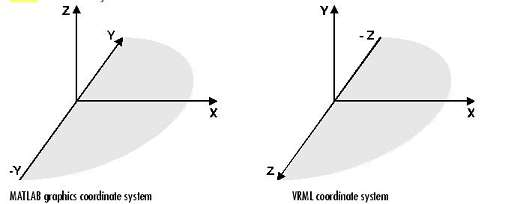
\includegraphics[scale=1]{Einleitung/matlabAndVrml.jpg}
	\caption[\matlab und \gls{vrml} Koordinatensystem]{\matlab und \gls{vrml} Koordinatensystem. Der Ursprung beider Systeme definieren den Mittelpunkt der Simulationsumgebung. Die X-Achsen zeigen in beiden Fällen Richtung Norden. Im \gls{vrml}-System zeigt die Z-Achse Richtung Ost, im \matlab -System zeigt dementsprechend die negative Y-Achse Richtung Ost.  In beiden Systemen liegt die Grundfläche auf dem Meeresboden. Somit zeigt die Z- bzw. Y-Achse vom Meeresboden aufwärts.}
	\label{Abb. 3}
\end{figure}
\todo{schöner evtl mit tik}

\subsection{Eingesetzte Software}
Neben den bereits erwähnten \matlab -Bibliotheken \textit{Simulink}, \textit{Graphics} und \textit{3D Animation} werden in dieser Arbeit noch weitere Bibliotheken verwendet.\\
Grundlegende geometrische Berechnungen, zum Beispiel \glspl{transform} in 2D und 3D oder auch Distanzberechnungen von Punkten werden mithilfe der freien Bibliotheken \textit{geom2d}\footnote{https://de.mathworks.com/matlabcentral/fileexchange/7844-geom2d} und \textit{geom3d}\footnote{https://de.mathworks.com/matlabcentral/fileexchange/24484-geom3d} durchgeführt.\\
Das Schätzverfahren nutzt die \textit{Optimization-Toolbox}\footnote{https://de.mathworks.com/products/optimization.html}, die Lösungen für verschiedene Minimierungs-, Maximierungs- und Optimierungsprobleme liefert.\\
Für die Kamerakalibrierung wurde die \textit{Computer Vision System Toolbox} genutzt. Die Toolbox bietet die einfach zu bedienende \textit{Camera Calibration App} mit der die intrinsischen Parameter bestimmt werden können.
Hilfestellung lieferte hierbei das dazugehörige Tutorial\footnote{https://de.mathworks.com/help/vision/ug/single-camera-calibrator-app.html}.\\